Trong phần này, tác giả đưa ra các định nghĩa chuẩn của một số thuật ngữ quan trọng liên quan đến đồ thị không thuần nhất. Minh họa trong hình 1. Bên cạnh đó bảng 1 tóm tắt các kí hiệu được sử dụng nhiều trong báo cáo để thuận tiện cho việc tra cứu nhanh.

\begin{definition}
\textbf{Đồ thị không đồng nhất.} Một đồ thị không đồng nhất được định nghĩa là một đồ thị $\pmb{\mathcal{G}} = (\pmb{\mathcal{V}}, \pmb{\mathcal{E}})$ với ánh xạ của loại nút $\phi: \pmb{\mathcal{V}} \to \pmb{\mathcal{A}}$ và ánh xạ của loại cạnh $\psi: \pmb{\mathcal{E}} \to \pmb{\mathcal{R}}$. $\pmb{\mathcal{A}}$ và $\pmb{\mathcal{R}}$ lần lượt là các tập loại nút và loại cạnh với $|\pmb{\mathcal{A}}| + |\pmb{\mathcal{R}}| > 2$.
\end{definition}

\begin{definition}
  \textbf{Metapath.} Một metapath $P$ được định nghĩa là một đường đi lập thành từ $A_1  \xrightarrow{R_1} A_2  \xrightarrow{R_2} ... \xrightarrow{R_l} A_{l+1}$ (viết tắt là $A_1 A_2 ... A_{l+1}$) mô tả một quan hệ tổng hợp $R = R_1 \circ R_2 \circ ... \circ R_l$ giữa các loại nút $A_1$ và $A_{l+1}$, trong đó $\circ$ là toán tử tổng hợp trên các quan hệ.
\end{definition}

\begin{definition}
  \textbf{Cấu hình metapath.} Cho một metapath $P$ của một đồ thị không đồng nhất, một cấu hình metapath $p$ của $P$ được định nghĩa là một dãy các nút trong đồ thị theo lược đồ được xác định bởi $P$.
\end{definition}

\begin{definition}
  \textbf{Lân cận dựa trên metaptah.} Cho một metapath $P$ của một đồ thị không đồng nhất, các lân cận dựa trên metapath $\pmb{\mathcal{N}}_\upsilon ^ P$ của một nút $\upsilon$ được định nghĩa là tập hợp các nút liên kết với nút $\upsilon$ qua các cấu hình metapath của $P$. Một lân cận được kết nối bởi hai cấu hình metapath khác nhau được đánh giá như hai nút khác nhau trong $\pmb{\mathcal{N}}_\upsilon ^ P$. Lưu ý rằng $\pmb{\mathcal{N}}_\upsilon ^ P$ bao gồm chính nút $\upsilon$ nếu $P$ đối xứng.

  Ví dụ, xem xét tập dữ liệu UATA trong hình 1, nghệ sĩ \textit{Queen} là một lân cân dựa trên metapath của người dùng \textit{Bob}. Hai nút này được kết nối thông qua cấu hình metapath \textit{Bob-Beatles-Rock-Queen}. Hơn nữa, chúng ta có thể tham chiếu tới \textit{Beatles} và \textit{Rock} như là các nút trung gian trên cấu hình metapath này.
\end{definition}

\begin{definition}
  \textbf{Đồ thị dựa trên metapath.} Cho một metapath $P$ của một đồ thị không đồng nhất $\pmb{\mathcal{G}}$, đồ thị dựa trên metapath $\pmb{\mathcal{G}}^P$ là một đồ thị được xây dựng bởi tất cả các cặp lân cận dựa trên metapath $P$ trong đồ thị $\pmb{\mathcal{G}}$. Lưu ý rằng $\pmb{\mathcal{G}}^P$ là đồng nhất nếu $P$ đối xứng.
\end{definition}

\begin{definition}
  \textbf{Biểu diễn đồ thị không đồng nhất.} Cho một đồ thị không đồng nhất $\pmb{\mathcal{G}} = (\pmb{\mathcal{V}}, \pmb{\mathcal{E}})$ với các ma trận thuộc tính nút $\pmb{X}_{A_i} \in \mathbb{R} ^ {|\pmb{\mathcal{V}}_{A_i}| \times d_{A_i}}$ của các loại nút $A_i \in \pmb{\mathcal{A}}$, biểu diễn đồ thị không đồng nhất là việc học các biểu diễn nút $d$ chiều $\pmb{h}_{\upsilon} \in \mathbb{R}^d$ với mọi $\upsilon \in \pmb{\mathcal{V}}$ với $d \ll |\pmb{\mathcal{V}}|$ có thể ghi lại thông tin cấu trúc và ngữ nghĩa liên quan đến $\pmb{\mathcal{G}}$.
\end{definition}

\begin{figure*}
  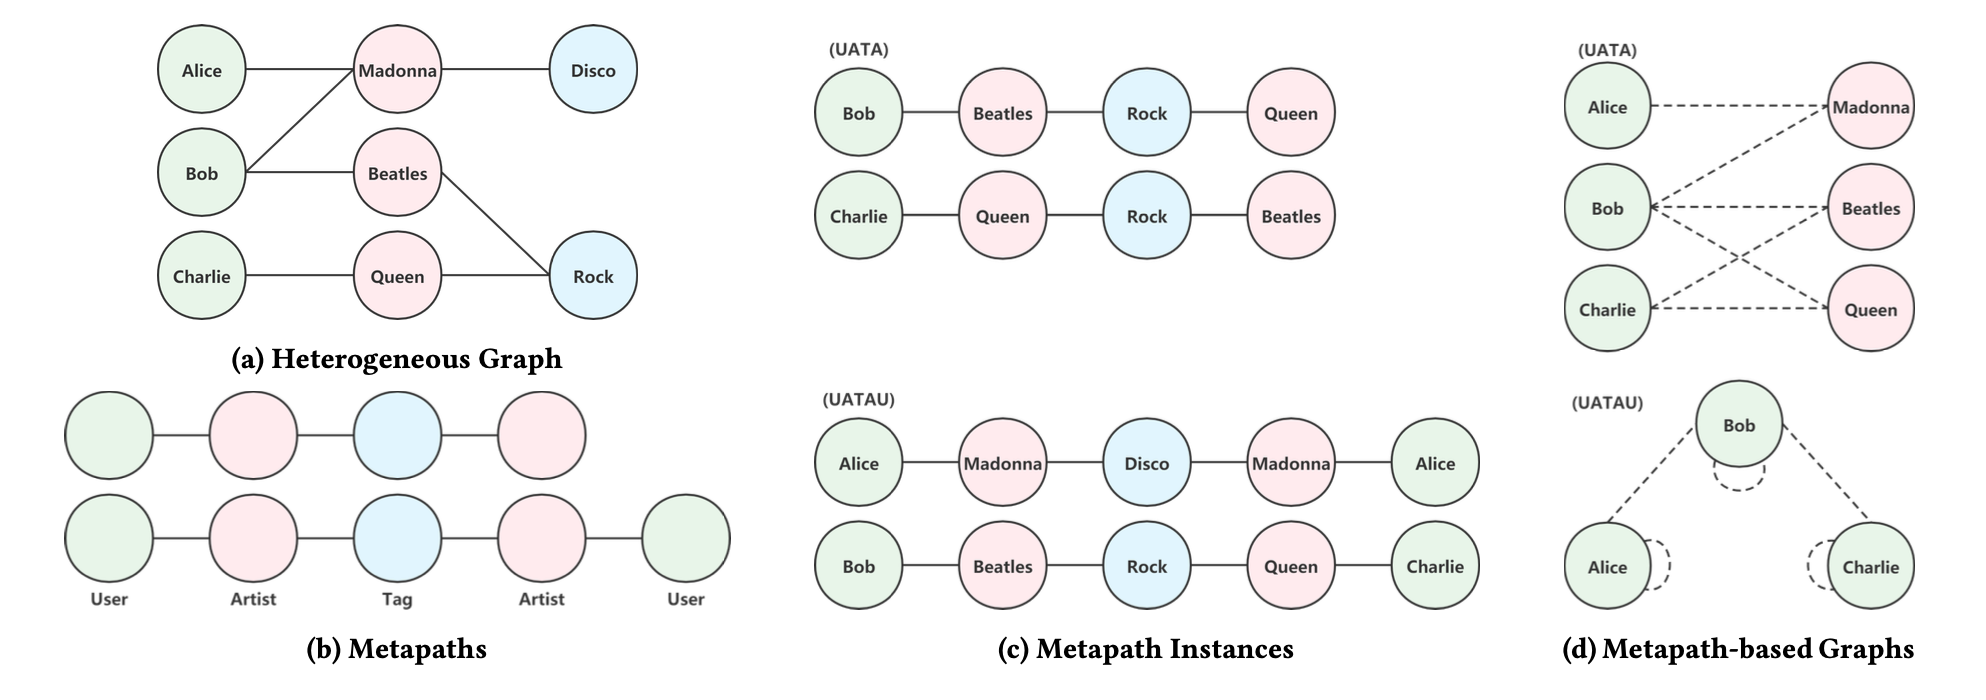
\includegraphics[width=\textwidth]{figs/fig1.png}
  \caption{Minh họa các thuật ngữ được định nghĩa trong Phần 2. (a) Một ví dụ về đồ thị không đồng nhất với ba loại nút (người dùng, nghệ sĩ, thẻ). (b) metapath Người dùng-Nghệ sĩ-Thẻ-Nghệ sĩ (UATA) và metapath Người dùng-Nghệ sĩ-Thẻ-Nghệ sĩ-Người dùng (UATAU). (c) Ví dụ các cấu hình metapath của UATA, UATAU. (d) Đồ thị dựa trên metapath cho UATA và UATAU.}
\end{figure*}



